\documentclass[10pt]{report}
\input{mahvPreamble}
\hypersetup{
  pdfauthor={Marco Arieli Herrera-Valdez},
  pdftitle={Notas de análisis de datos de transientes de Calcio obtenidos en el laboratorio de T. Fiordelisio. }
  pdftex,
  colorlinks=true,
  urlcolor=Bittersweet,
  linkcolor=blue,
  pdftoolbar=true,
  pdfmenubar=true,
  citecolor=Purple,
  filecolor=blue, 
}


\begin{document}

Normalization of {\calcium} traces:
\begin{equation}
F_{norm}= \frac{F - F_{min}}{F_{min}}
\label{FminNormalization}
\end{equation}

\begin{figure}
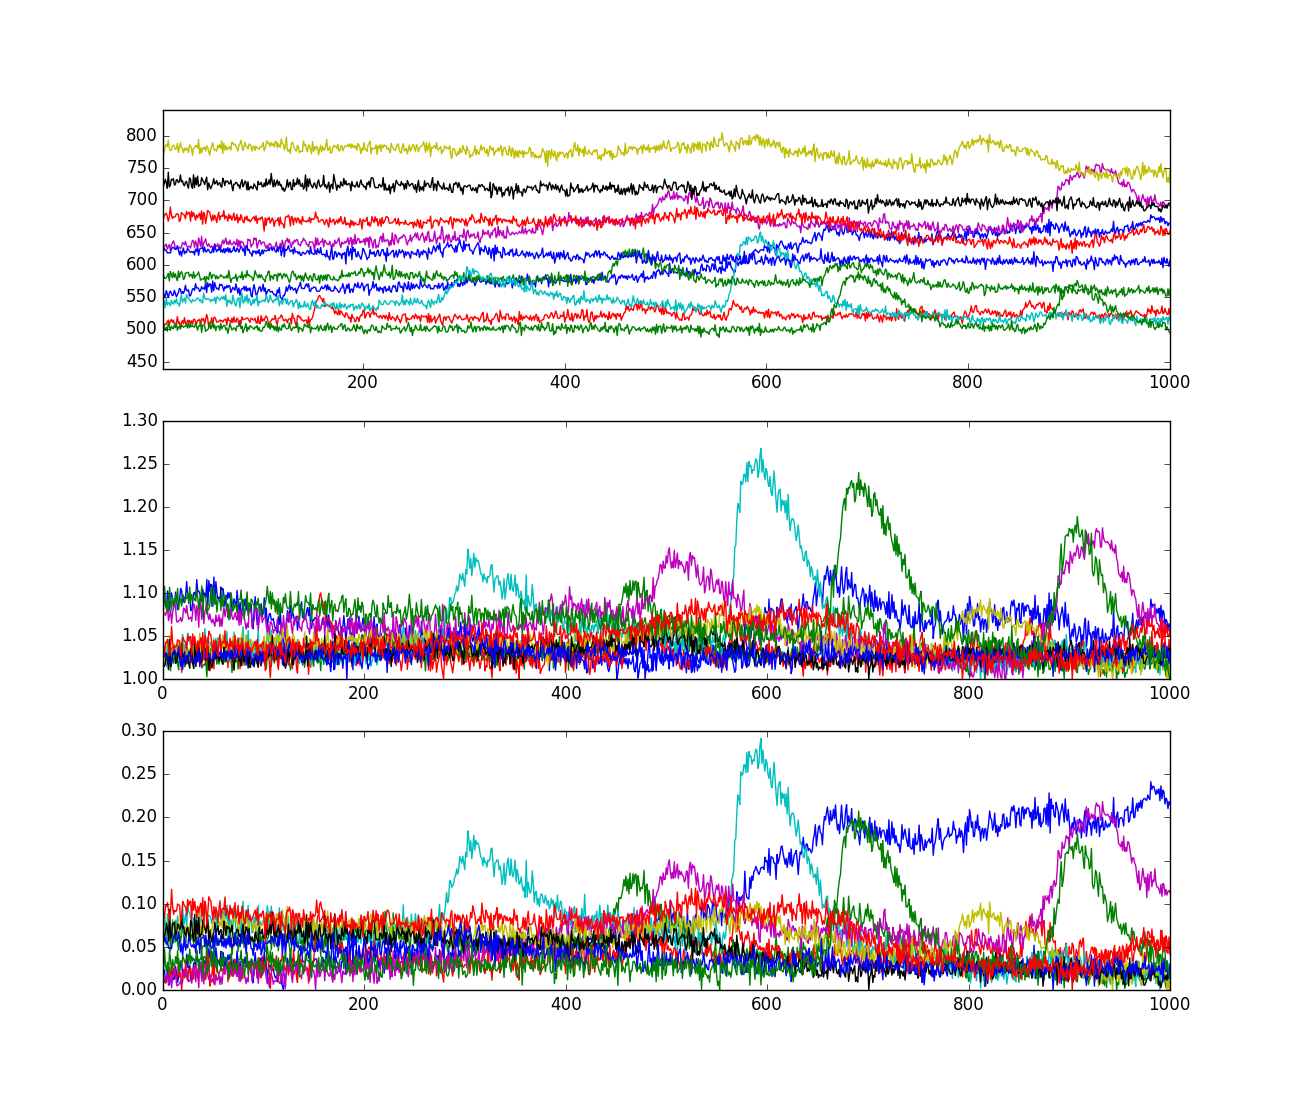
\includegraphics[width=\textwidth]{figures/F-FminOverFmin_CtxDaniel.png}
\caption{From top to bottom. Original {\calcium} traces (top), de-bleached traces with a custom-written program in Igor (middle), and normalized traces only using $F_{min}$ as in equation \eqref{FminNormalization} (bottom). Interpretation (??).}
\end{figure}

\begin{figure}
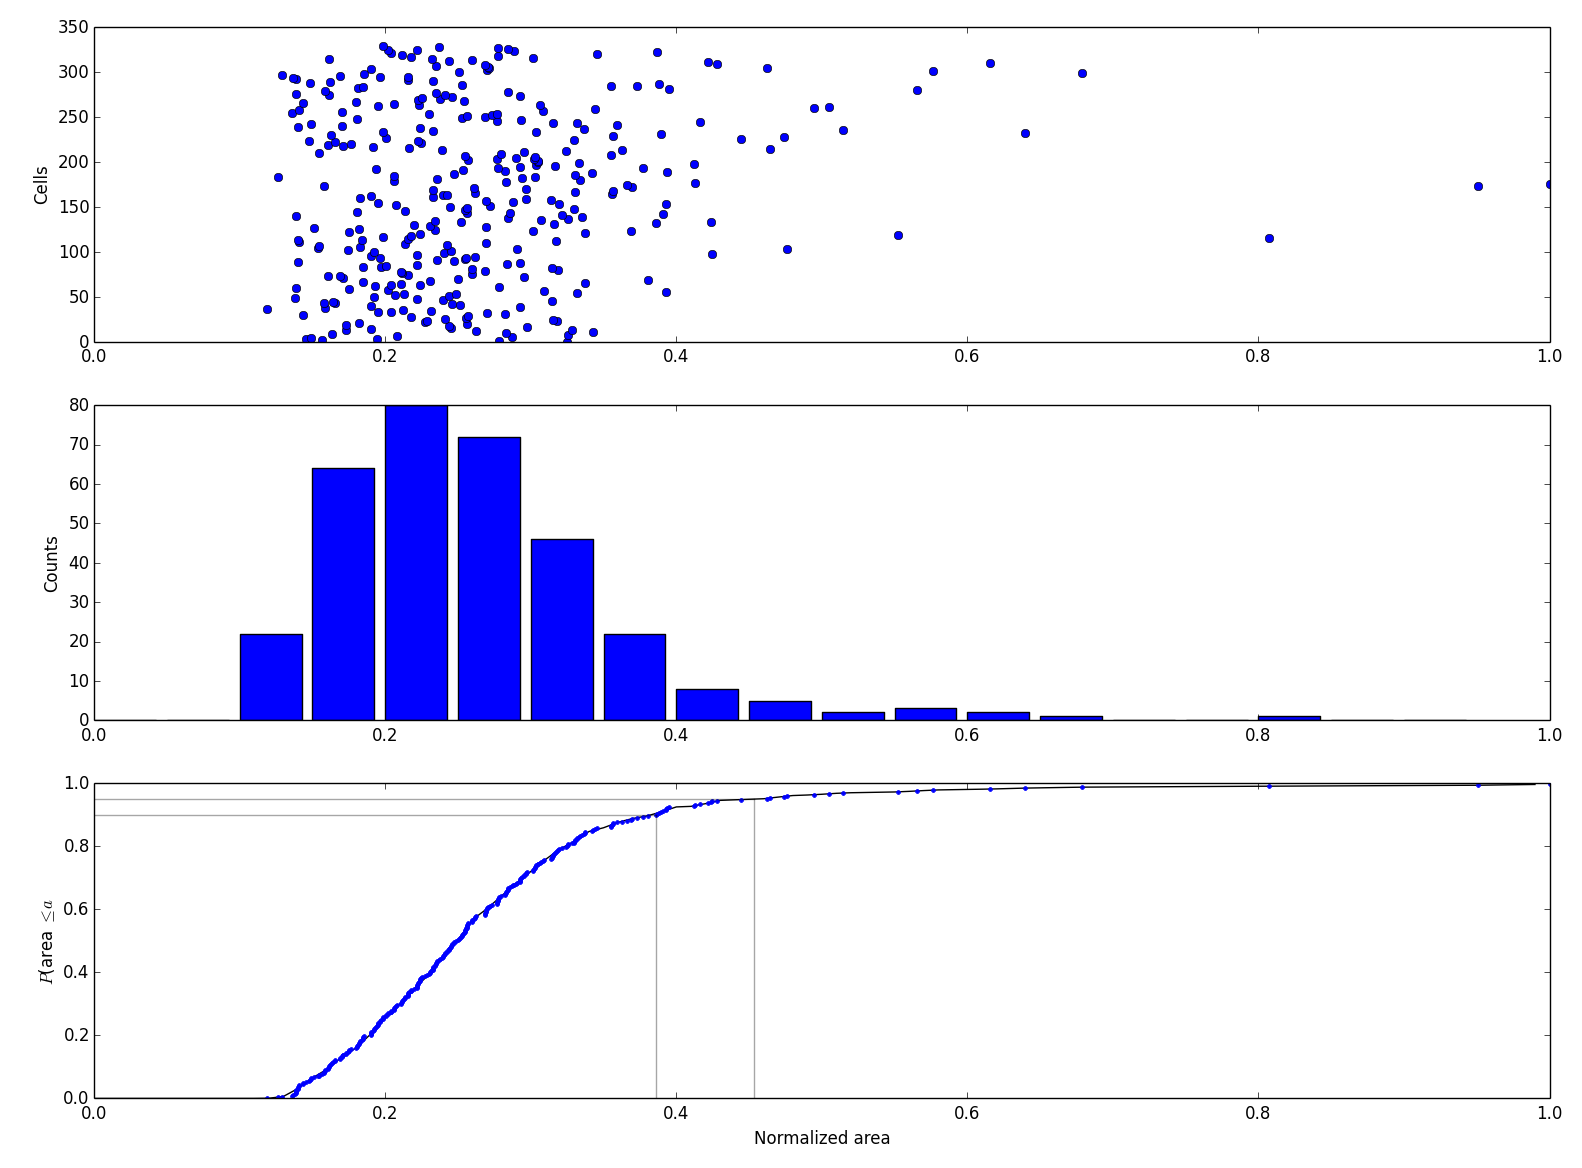
\includegraphics[width=\textwidth]{figures/AreasNormalizadas_CtxDaniel.png}
\caption{Area under the curve for each of the traces in the data set.  Two thresholds for significatively high area were used, }
\end{figure}


\end{document}